% lec1.tex 
\chapter{Power Series}
\lecture{1}{08:06 AM Mon, Sep 29 2025}{} 

\begin{definition}[Power Series]
  A power series is a formal series of the form 
  $\sum_{n=0}^{\infty} a_{n}z^{n} $, where $a_{n} \in  \CC $ for all
  $n \in \NN_0$. \\
  More generally, given $z_0 \in \CC  $, a power series 
  centered at  $z_0 $ is a formal series of the form: 
  \[
  \sum_{n=0}^{\infty} a_{n}(z-z_0) ^{n},
  \]
  where $a_{n} \in \CC  \quad (\forall n \in \NN_0)  $ 
\end{definition}
\begin{remark}
  The set of all complex power series 
  (centered at $0 $) is denoted by 
  $\CC \left[ [z] \right] $. More generally, given
  $z_0 \in  \CC  $, the set of all complex power series centered
  at $z_0 $ is denoted by $\CC 
  \left[ [z-z_0] \right]
  $. 
\end{remark}
\noindent  \textcolor{larratBicep!10!brown}{
  \uline{
\large\emph{ \ding{43} Operations on Formal Power Series:}
  }
}\\
Given $z_0 \in  \CC  $, we equip $\CC \left[ \left[ z-z_0 \right] \right] $.
with the following operations: 
\begin{itemize}
  \item[\ding{172}]\textbf{Additions:} For all $(a_{n}) _{n \in \NN_0}, (b_{n}) _{n \in \NN_0} \subset   \CC$:
  \[
  \sum_{n=0}^{\infty} a_{n}(z-z_0) ^n + \sum_{n=0}^{\infty} b_{n}(z-z_0) ^n = 
  \sum_{n=0}^{\infty} (a_{n} + b_n ) (z-z_0) ^n.
  \]
\item[\ding{173}]\textbf{Multiplication} 
  \[
  \sum_{n=0}^{\infty} a_{n}(z-z_0) ^n  \times \sum_{n=0}^{\infty} 
  b_n (z-z_0) ^n = 
  \sum_{n=0}^{\infty} c_{n} (z-z_0) ^n,
  \]
  where, $c _n := \sum_{k=0}^{n} a_{k} b_{n-k} $  for all $n \in \NN_0 $.
  Also $(c_{n}) _{n \in \NN} $ is called the covolution of the two sequences
  $(a_{n}) _{n \in \NN_0} $ and $(b_{n}) _{n \in \NN_0} $ .
\item[\ding{174}]
   \textbf{Scalar Multiplication:} For all $\lm \in  \CC  $, and all $(a_{n}) _{n \in \NN_0} \subset   \CC  $:
   \begin{align*}
   \lm \sum_{n=0}^{\infty} a_{n}(z-z_0) ^n  = 
   \sum_{n=0}^{\infty} (\lm a _n ) (z-z_0) ^n.
   \end{align*}
\end{itemize}
It's straightforward to verify that $\CC \left[ \left[ z-z_0 \right] \right] $  equipped with these operations 
forms a commutative algebra over $\CC  $. The Multiplicative identity is the constant power series:
\[
1 = 1 + 0 \cdot ( z-z_0)  + 0 \cdot (z-z_0) ^2 + \hdots 
\]
\begin{definition}[Domain of Convergence]
The domain of convergence of a power series 
$\sum_{n=0}^{\infty} a_n (z-z_0) ^n  $ is the set of all points $z \in  \CC  $ for which 
the series converge. The structure of this domain is very specific. Its a disk (possibly with 
some points in its boundary) centered at $z_0$.
\end{definition}

\begin{proposition}[Abel's Lemma]
  Let $\sum_{n=0}^{\infty} a_n (z-z_0) ^n  $ be a power
  series and let $z_1 \in  \CC \backslash 
  \left\{ z_0 \right\}$. Suppose that the sequence
  $\left\{ a_{n}(z_1-z_0) ^n  \right\}_{n \in \NN_0}$ is 
  bounded. Then, the power series in question converges
  absolutely (so converges) for every $z \in \CC$, such that: 
  \[
  \left| z-z_0 \right| <  \left| z_1-z_0 \right|
  \]
\end{proposition}
\begin{proof}
  By hypothesis, $\exists M > 0 $ such that $\forall n \in  \NN_0$: 
  \[
  \left| a_n (z_1-z_0) ^n  \right| \leq M
  \]
  Then, for all $z \in \CC  $ such that $\left| z-z_0 \right| < \left| z_1-z_0 \right|$ we have:
  \begin{align*}
    \left| a_n (z-z_0) ^n  \right| &= 
    \underbrace{
    \left| a_n (z_1-z_0) ^n  \right|
    }_{ \leq  M} 
    \cdot 
    \underbrace{
    \left| \frac{z - z_0}{z_1-z_0} \right|^n 
    }_{< 1} 
    \\
    & \leq  M 
    \underbrace{
    \left| \frac{z-z_0}{z_1-z_0} \right|^n 
    }_{ < 1}. 
  \end{align*}
  Since $\left| \frac{z-z_0}{z_1-z_0} \right| <  1$ then the geometric series 
  \[
  \sum_{n=0}^{\infty} M \left| \frac{z-z_0}{z_1-z_0} \right|^n  \text{ Converges } .
  \]
  Thus, the series $\sum_{n=0}^{\infty} \left| a_n (z-z_0) ^n  \right| $ also converges,
  that is $\sum_{n=0}^{\infty} a_n (z-z_0) ^n  $ is absolutely convergent.
\end{proof}

\begin{corollary}[]
Let $\sum_{n=0}^{\infty} a_n (z-z_0) ^n  $ be a power series which converges
at some  $z = z_1 \in \CC  \backslash \left\{ z_0 \right\} $. Then the power series
in question converges absolutely (so converges), for every $z \in \CC  $ such that: 
\[
\left| z-z_0 \right| <  \left| z-z_1 \right| 
\quad  \quad  \quad 
\quad \quad \quad 
\quad \quad \quad 
\quad \quad \quad 
\begin{tikzpicture}[overlay]
  \draw[fill=gray, opacity=0.4] (0, 0) circle (1cm);
  \node[anchor=north] at (0,0) { $z_0 $ };
  \node[] at (0,0) {\tiny $\times   $  };
  \node[anchor=south west] at (30:1) { $z_1 $ };
  \node[anchor=south east ] at (70:0.5) { $z $ };
  \node[] at (70:0.5) {\tiny$\times $  };
  \node[] at (30:1) {\tiny $\times   $ };
\end{tikzpicture}
\]

\begin{center}
\end{center}
\end{corollary}

\begin{proof}
$\sum_{n=0}^{\infty} a_n (z_1-z_0) ^n  $ converges implies  that $a_n (z-z_0) ^n  \rightarrow 0 $  
as $n \rightarrow + \infty  $, which implies that the sequence $\left\{ a_n (z_1-z_0) ^n  \right\}_{n \geq 0} $ is bounded.
\it Proposition 1.0.1 \normalfont permits us to conclude the required result.
\end{proof}
\begin{theorem}[Radius of Convergence]
  Let $\sum_{n=0}^{\infty} a_n (z-z_0) ^n  $ be a power series. Then there exists a unique $R \in \left[ 0, \infty  \right] $, 
  called the radius of convergence with the following properties: 
  \begin{enumerate}
    \item[\ding{172}]The power series converges absolutely for every $z \in \CC  $ satisfying $\left| z-z_0 \right| <  R $.
    \item[\ding{173}] The power series diverges for every $z \in \CC  $ satisfying $\left| z-z_0 \right|> R $. 
      The disk $D(z_0, R)  = \left\{ z \in  \CC : \quad \left| z-z_0 \right|< R \right\} $ is called
      the disk of convergence.
  \end{enumerate}
\end{theorem}

\begin{proof}
Define the set $A \subset \RR_{ \geq 0} $ of nonegative real numbers for which 
the sequence $\left\{ \left| a_n  \right| r^{n} \right\}_{n \in \NN_0}$  is bounded.
\[
A := 
\left\{ r \geq 0: \quad \sup_{n \in  \NN_0}  \left| a_n  \right|r^{n} < \infty  \right\}
\]
we have $A \neq \emptyset  $ because $ 0 \in  A $. 
Define $R := \sup_{} A \in \left[ 0, \infty  \right]$, we now show that $R $ has the stated
properties.
\begin{enumerate}
  \item[\ding{50}\ding{172}] Let $z \in  D(z_0, R)  $. By definition of the supremum, there exists $r \in  A $, (i.e., 
  $\left| a_n  \right|r^{n} $ is bounded) such that $\left| z-z_0 \right| <  r \leq R$. Since 
  $\left| z-z_0 \right|<  r $  and $\left\{ \left| a_n  \right|r^n  \right\}_{n \geq 0}$ is bounded, 
  then by Abel's lemma, we deduce that the series $\sum_{n=0}^{\infty} a_n (z-z_0) ^n  $ converges 
  absolutely.
\item[\ding{50}\ding{173}]Let $z \in  \CC  $ such that $\left| z-z_0 \right| > R $, suppose for contradictions that the power 
   series converges at $z $. Then by the \it Corollary 1.0.2\normalfont, it would converge absolutely for any
   $\omega  $ with $\left|  \omega - z_0 \right|<   \left| z-z_0 \right|$. In particular, for any $r $ such that: 
   \[
   R < r <  \left| z-z_0\right|
   \]
   the series would converge at points on the circle $C(z_0, r)  $, implying $r \in  A$. This contradicts 
   the fact that $R = \sup_{} A $. Therefore, the power series diverges.
\end{enumerate}
\uline{\ding{50}~The Uniqueness of R:} \\
If another $R' \in \left[ 0, \infty  \right] $ satisfies
the same properties, a point $z $ such that $\left| z-z_0 \right| $ lies between $R $ 
and $R' $ would lead to a contradiction regarding the convergence or divergence of the power series.
\end{proof}
\section{Formulas for Calculating the Radius of Convergence}
\begin{proposition}[Hadamard's Formula]
  Let $\sum_{n=0}^{\infty} a_n (z-z_0) ^n  $ be a power series centered at 
  $z_0 \in \CC$. Denote by $R $ its radius of convergence. Then: 
  \[
  \frac{1}{R} = 
  \lim_{n \to \infty} \sup_{} 
  \sqrt[n]{\left| a_n  \right|}
  \]
  with the convention $\frac{1}{0} = \infty  $  and $\frac{1}{\infty }= 0 $ 
\end{proposition}
\begin{proof}
  Let $L := \lim_{n \to \infty} \sup_{} \left| a_n  \right|^{\frac{1}{n}} \in \left[ 0, \infty  \right]$. 
  We must show that $R = \frac{1}{L} $. Let $z \in  \CC \backslash \left\{ z_0 \right\} $, we distinguish 
  three cases:
  \begin{itemize}
    \item[\ding{50}\ding{172}] If $L = 0 $. In this case, we have:
      \[
        0 \leq  \lim_{n \to \infty} \inf_{} \left| a_n  \right|^{\frac{1}{n}} \leq 
        \lim_{n \to \infty} \sup_{} 
        \left| a_n  \right|^{\frac{1}{n}} = 0
      \]
      Thus, $\lim_{n \to \infty} \inf_{} \left| a_n  \right|^{\frac{1}{n}} = \lim_{n \to \infty} \sup_{} 
      \left| a_n  \right|^{\frac{1}{n}} = 0$.
  This implies that $\lim_{n \to \infty} \left| a_n  \right|^{\frac{1}{n}} $ exists and equals to $0$, so for all
  $n $ sufficiently large, we have: 
  \[
    \left| a_n  \right|^{\frac{1}{n}} <  
    \frac{1}{2 \left| z-z_0 \right|} ;
  \]
  That is,
  \[
  \left| a_n (z-z_0) ^n  \right| <  
  \frac{1}{2^n }.
  \]
  Since the geometric series $\sum_{n=1}^{\infty} \frac{1}{2^{n}} $ converges
  then the series $\sum_{n=0}^{\infty} \left| a_n (z-z_0) ^n  \right| $ converges 
  $\forall z \in  \CC  $, thus $R = +\infty = \frac{1}{L}$ 
\item[\ding{50} \ding{173}] If $L = +\infty $, we have $L = \lim_{n \to \infty} \sup_{} \left| a_n  \right|^{\frac{1}{n}} = +\infty $ is 
   equivallent to the fact that the sequence $\left\{ \left| a_n  \right|^{\frac{1}{n}} \right\}_{n \in \NN} $ is bounded.
   Therefore, the sequence: 
   \[
   \left| a_n (z-z_0) ^n \right|^{\frac{1}{n}} = 
   \left| a_n  \right|^{\frac{1}{n}} \left| 
   z-z_0\right| 
   \]
   is also unbounded. This implies that $\left| a_n (z-z_0) ^n  \right| $ is unbounded, thus 
   $\left| a_n (z-z_0) ^n  \right|$ does not converge to $0 $ as $n \rightarrow \infty  $. Hence 
   $\sum_{n=0}^{\infty} a_n (z-z_0) ^n  $ diverges. Hence $R = 0 $.
 \item[\ding{50} \ding{174}] If$L \in  (0, \infty ) $. Let $z \in  \CC  $. We consider two subcases:
     \begin{itemize}
       \item[\ding{182}] If $ \left| z-z_0 \right| < \frac{1}{L}$. Choose $r $ such that 
       $\left| z-z_0 \right|<  r < \frac{1}{L} $, thus $L < \frac{1}{r} $. By defintion of a $\lim_{n \to \infty} \sup_{}  $,
       for all $n $ sufficiently large we have: 
       \[
       \left| a_n  \right|^{\frac{1}{n}} <  \frac{1}{r},
       \]
       which implies that: 
       \[
       \left| a_n (z-z_0) ^n  \right| <  
       \underbrace{
         \left( 
           \frac{\left| z-z_0 \right|}{r}
         \right)^n 
       }_{<  1}. 
       \]
       Since $\left| \frac{z-z_0}{r} \right| <  1$, the geometric series $\sum_{n=0}^{\infty} \left| \frac{z-z_0}{r} \right|^n $ converges. By comparison, the power series $\sum_{n=0}^{\infty} a_n (z-z_0) ^n  $ converges absolutely.
     \item[\ding{183}] 
        If $(\left| z-z_0 \right| > \frac{1}{L})  $. In this case, we have:
        \begin{align*}
        \lim_{n \to \infty} \sup_{} 
        \left| a_n (z-z_0) ^n  \right|^{\frac{1}{n}} & = 
        \lim_{n \to \infty} \sup_{} 
        \left( 
          \left| a_n  \right|^{\frac{1}{n}} \left| z-z_0 \right| 
        \right) \\
        &=
        L \left| z-z_0 \right| > 1
        \end{align*}
        Thus, $\left\{ a_n (z-z_0) ^n  \right\}_{n \in  \NN} $  is unbounded, hence 
        $\left| a_n (z-z_0) ^n  \right| $  does not converge to zero as $n \rightarrow \infty  $, 
        implying that $\sum_{n=0}^{\infty} a_n (z-z_0) ^n  $  diverges. Therefore:
        \[
        R = \frac{1}{L}.
        \]
     \end{itemize}
  \end{itemize}
\end{proof}
% end of file
